
\documentclass[14pt]{extarticle}
\usepackage{graphicx}
\usepackage{pdfpages}
\usepackage[margin=1in]{geometry}

\graphicspath{ {./images/} }

\begin{document}
    \pagenumbering{arabic}
    \pagestyle{plain}

    \title{\Huge Assignment 2\\ Computer Networks}
    \author{\huge Vikas Gola}
    \maketitle
    \newpage

    \noindent
    \textbf{\large Question 1}
    Examine the following files in Linux and find out what is the purpose served by each. 
    Write at least two sentences mentioning the purpose of each.
    \begin{itemize}
        \item /etc/hosts
        \item /etc/sysconfig/network
        \item /etc/sysconfig/network-scripts/ifcfg-eth0
        \item /etc/default-route
        \item /etc/resolv.conf
        \item /etc/nsswitch.conf
    \end{itemize}
    \textbf{\large Answer}
    \begin{itemize}
        \item \textbf{/etc/hosts}
        \\This file is used to find the IPA of corresponding hostname and to do that 
        it has mapping from hostname to IP address which will be accessed whenever corresponding hostname tried to be reach
        on the machine. Whenever some hostname is requested by user first this file will run and try to find IP address
        of destination address that has to be reached and if no IPA is founded then request goes to DNS to do the same thing.
        \item \textbf{/etc/sysconfig/network}
        \\This file contains the settings or network configuration that is needed on your server.  
        \item \textbf{/etc/sysconfig/network-scripts/ifcfg-eth0}
        \\This file contains the details of your network interface like should it start onboot or not,name of device, device address etc.   
        \item \textbf{/etc/default-route}
        \\ File does not exist. Didn't find anything on internet also.
        \item \textbf{/etc/resolv.conf}
        \\This file contains and used to find the IP address of hostname by system. 
        \item \textbf{/etc/nsswitch.conf}
        \\This file is configuration file which configures the service to use for finding password, groups and hostnames.
    \end{itemize}
    \vspace{1cm}

    
    \noindent
    \textbf{\large Question 2}
    Display the file /etc/services on your screen, using appropriate Linux command. What is the use of
/etc/services file? Which layer in the TCP/IP protocol stack do you think would make use of this file
? Are the port numbers shown in this file well-known port numbers or ephemeral port numbers ? Why
are they so ? Give appropriate reasoning for your answer\\[10pt]
    \textbf{\large Answer}
    This file is one most important file as it contains details about all service on system which port it use, which protocol it is using and aliases to services.
    This file is used in the Transport Layer Protocol(TLP). 
    All port numbers on this file are well known port numbers and the reason for this is that all service has to respond to some requests and so answer to request can be easily handle by OS or system
    if it already no where to or which service to serve the request that can find service easily by mapped well known port numbers in this file.\\[8pt]
    \vspace{1cm}


    \noindent
    \textbf{\large Question 3}
    Read the man pages for the following programs:
    \begin{itemize}
        \item arp
        \item arping
        \item ifconfig
        \item tcpdump
        \item ping
        \item netstat
        \item route
    \end{itemize}
    Find out the the purpose of each of these commands. In those cases whereever applicable, list out
    the application layer, transport layer and the network layer protocols used by each command. Pre-
    pare a table with the following columns to answer your question viz. command name, Purpose, Trans-
    port layer protocol used, Network layer protocol used.\\[10pt]    
    \textbf{\large Answer}
    Following table list out the layers used by given the commands:
    \begin{table}[!h]
        \begin{center}
            \begin{tabular}{c|c|c|c}
                \textbf{Commands} & \textbf{Application}  & \textbf{Transport} & \textbf{Network} \\ 
                & \textbf{Layer Protocol} & \textbf{Layer Protocol} & \textbf{Layer Protocol}  \\ 
                \hline
                arp & NA & NA & ARP \\
                \hline
                arping & NA & NA & ARP\\
                \hline
                ifconfig & NA & NA & IP\\
                \hline
                tcpdump & NA & TCP & ARP\\
                \hline
                ping & NA & ICMP & IP\\
                \hline
                netstat & NA & TCP & IP\\
                \hline
                route & NA & UDP & IP
            \end{tabular}    
        \end{center}
    \end{table}
    \begin{itemize}
        \item \textsf{arp} 
        Stands for "Address Resolution Protocol." 
        ARP is a protocol used for mapping an IP address to a computer connected to a local network LAN. 
        Since each computer has a unique physical address called a MAC address, the ARP converts the IP address to the MAC address. 
        This ensures each computer has a unique network identification.
        \item \textsf{arping}
        It's purpose is to send ARP request on the local network and to print received responses.
        \item \textsf{ifconfig}
        This command is used to get info about network interfaces.
        This command can also be used to configure, disable and enable a network interface.
        \item \textsf{tcpdump}
        This command is used to capture packets on network and analyze different network interfaces. 
        \item \textsf{ping}
        This command is used to send ICMP request to the given ip address and print the response.
        \item \textsf{netstat}
        This command is used to get network details and statistics. Also, used to get routing table of network.
        \item \textsf{route}
        Main use of route command is used to edit and get the routing table.
    \end{itemize}
    
    \vspace{1cm}


    \noindent
    \textbf{\large Question 4}
    This exercise is a simple exercise that only requires you to capture the tcpdump traffic. The problem
requires you to either use two virtual machines on your laptop or two different machines in the computer
lab - ask the administrator for the host name of both the machines, if so. Then run the tcpdump command
on one machine say PC1 (saving the output for your lab report) so that it monitors all the packets that
contain the IP address of PC2 only and none else. Next, open a new terminal window on PC1 and execute
a ping command to PC2. It may be necessary to press Ctrl-C to terminate the tcpdump session. It may
sometimes be best to simply redirect the output of tcpdump straight to a file and view it afterward with
the more command or a text editor. Find out how can you do so.\\[10pt]
    \textbf{\large Answer}
    The output of tcpdump has been redirect to file using the comand \textsf{sudo tcpdump icmp $>$ ping.txt} and the output in the file is \\
    01:38:38.435936 IP 10.10.42.119 $>$ 10.10.60.30: ICMP echo request, id 6716, seq 131, length 64\\
    01:38:38.435987 IP 10.10.60.30 $>$ 10.10.42.119: ICMP echo reply, id 6716, seq 131, length 64\\
    01:38:39.438031 IP 10.10.42.119 $>$ 10.10.60.30: ICMP echo request, id 6716, seq 132, length 64\\
    01:38:39.438081 IP 10.10.60.30 $>$ 10.10.42.119: ICMP echo reply, id 6716, seq 132, length 64\\
    01:38:40.439569 IP 10.10.42.119 $>$ 10.10.60.30: ICMP echo request, id 6716, seq 133, length 64\\
    01:38:40.439620 IP 10.10.60.30 $>$ 10.10.42.119: ICMP echo reply, id 6716, seq 133, length 64\\
    01:38:41.438408 IP 10.10.42.119 $>$ 10.10.60.30: ICMP echo request, id 6716, seq 134, length 64\\
    01:38:41.438458 IP 10.10.60.30 $>$ 10.10.42.119: ICMP echo reply, id 6716, seq 134, length 64\\
    \\
    \vspace{1cm}

    \noindent
    \textbf{\large Question 5}
    Run the command tcpdump -enx -w exe5.out. Do you see any output on the screen ? Why ?\\[10pt]
    \textbf{\large Answer}
    We don't see any output on screen on running the command \textsf{tcpdump -enx -w tcpdump.out} because all the output and details of captured 
    packet has been write to file tcpdump.out file.\\[8pt]
    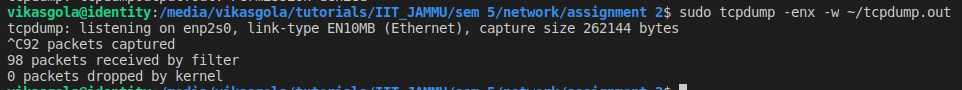
\includegraphics[scale=0.48]{5}
    \vspace{1cm}

    \noindent
    \textbf{\large Question 6}
    This question is in continuation of the question no 5. Run telnet remote host. remote host is the host
name of either another virtual machine in your machine or it is the host name of any other machine in
the network used in the lab (Ask the lab technical suport staff about the name of other machine). This
command would generate some TCP traffic. After you login the remote machine, terminate the telnet
session and terminate the tcpdump program.
Next, you will use wireshark to open the packet trace captured by tcpdump and analyze the captured
packets. To do this, run wireshark -r exe5.out \&. The wireshark Graphical User Interface (GUI) will
pop up and the packets captured by tcpdump will be displayed. For your report, you need to save any
one of the packets that contain the link, IP, and TCP headers. Carry out the following instructions.
    \begin{itemize}
        \item Click on a TCP packet from the list of captured packets in the wireshark window. Then go to the
        Edit menu and choose Mark Frame.
        
        \item Go to the File menu and choose Print. In the Wireshark:Print dialog that pops up, check File,
       Plain Text, Expand all levels, Print detail and supress unmarked frames. Then, enter the output
       text file name, e.g., headers.txt, and click the OK button. The marked packet is now dumped into
       the text file, with a detailed list of the name and value of every field in all the three headers.
    \end{itemize}
    Now answer the following questions:
    \begin{itemize}
        \item Draw the format of the packet you saved, including the link, IP, and TCP headers (See Figs in the
        handouts given to you for reference), and identify the value of each field in these headers. Express
        the values in the decimal format. 
        \item What is the value of the protocol field in the IP header of the packet you saved? What is the use
        of the protocol field?
    \end{itemize}
    \textbf{\large Answer}
    The header pdf file has been included in this pdf that is on page 9(headers.pdf).
    \begin{itemize}
        \item \textsf{Link Header Frame}
            \begin{itemize}
                \item Destination Address: HewlettP\_2d:7f:92 (a0:8c:fd:2d:7f:92)
                \item Source Address: Cisco\_af:0c:44 (a0:3d:6f:af:0c:44)
            \end{itemize}
        
        \item \textsf{IP Header} 
            \begin{itemize}
            \item Version: 4
            \item Header Length: 20 bytes
            \item 0x10 (DSCP: Unknown, ECN: Not-ECT)
            \item Total Length: 52
            \item Identification: 0xc88a (51338)
            \item Flags: 0x4000, Don't fragment \\
                0... .... .... .... = Reserved bit: Not set\\       
                .1.. .... .... .... = Don't fragment: Set\\        
                ..0. .... .... .... = More fragments: Not set\\        
                ...0 0000 0000 0000 = Fragment offset: 0\\    
            \item Time to live: 63    
            \item Protocol: TCP (6)    
            \item Header checksum: 0xf880 [validation disabled]    [Header checksum status: Unverified]    
            \item Source: 10.10.42.119    
            \item Destination: 10.10.60.30
        \end{itemize}
        \item \textsf{TCP Header}
            \begin{itemize}
                \item Source Port: 23    
                \item Destination Port: 54448    {[Stream index: 2]}    {[TCP Segment Len: 0]}    
                \item Sequence number: 1957099778    {[Next sequence number: 1957099778]}    
                \item Acknowledgment number: 1471419429 1000 .... = 
                \item Header Length: 32 bytes (8)    
                \item Flags: 0x010 (ACK)\\        
                000. .... .... = Reserved: Not set\\        
                ...0 .... .... = Nonce: Not set\\        
                .... 0... .... = Congestion Window Reduced (CWR): Not set\\        
                .... .0.. .... = ECN-Echo: Not set\\        
                .... ..0. .... = Urgent: Not set\\        
                .... ...1 .... = Acknowledgment: Set\\
                .... .... 0... = Push: Not set\\
                .... .... .0.. = Reset: Not set\\
                .... .... ..0. = Syn: Not set\\        
                .... .... ...0 = Fin: Not set\\        
                {[TCP Flags: ·······A····]}    
                \item Window size value: 227
                \item Checksum: 0x544d {[unverified]}    {[Checksum Status: Unverified]}    
                \item Urgent pointer: 0    
                \item Options: (12 bytes), No-Operation (NOP), No-Operation (NOP), Timestamps\\
                TCP Option - No-Operation (NOP)\\            
                Kind: No-Operation (1)\\        
                TCP Option - No-Operation (NOP)\\            
                Kind: No-Operation (1)\\        
                TCP Option - Timestamps: TSval 2224601295, TSecr 3851670941\\            
                Kind: Time Stamp Option (8)            Length: 10            
                Timestamp value: 2224601295            Timestamp echo reply: 3851670941
            \end{itemize}
    \end{itemize}

    The value of protocol field in IP header is "TCP". This field tell us which Transport layer protocol has been used in packet.\\[10pt]
    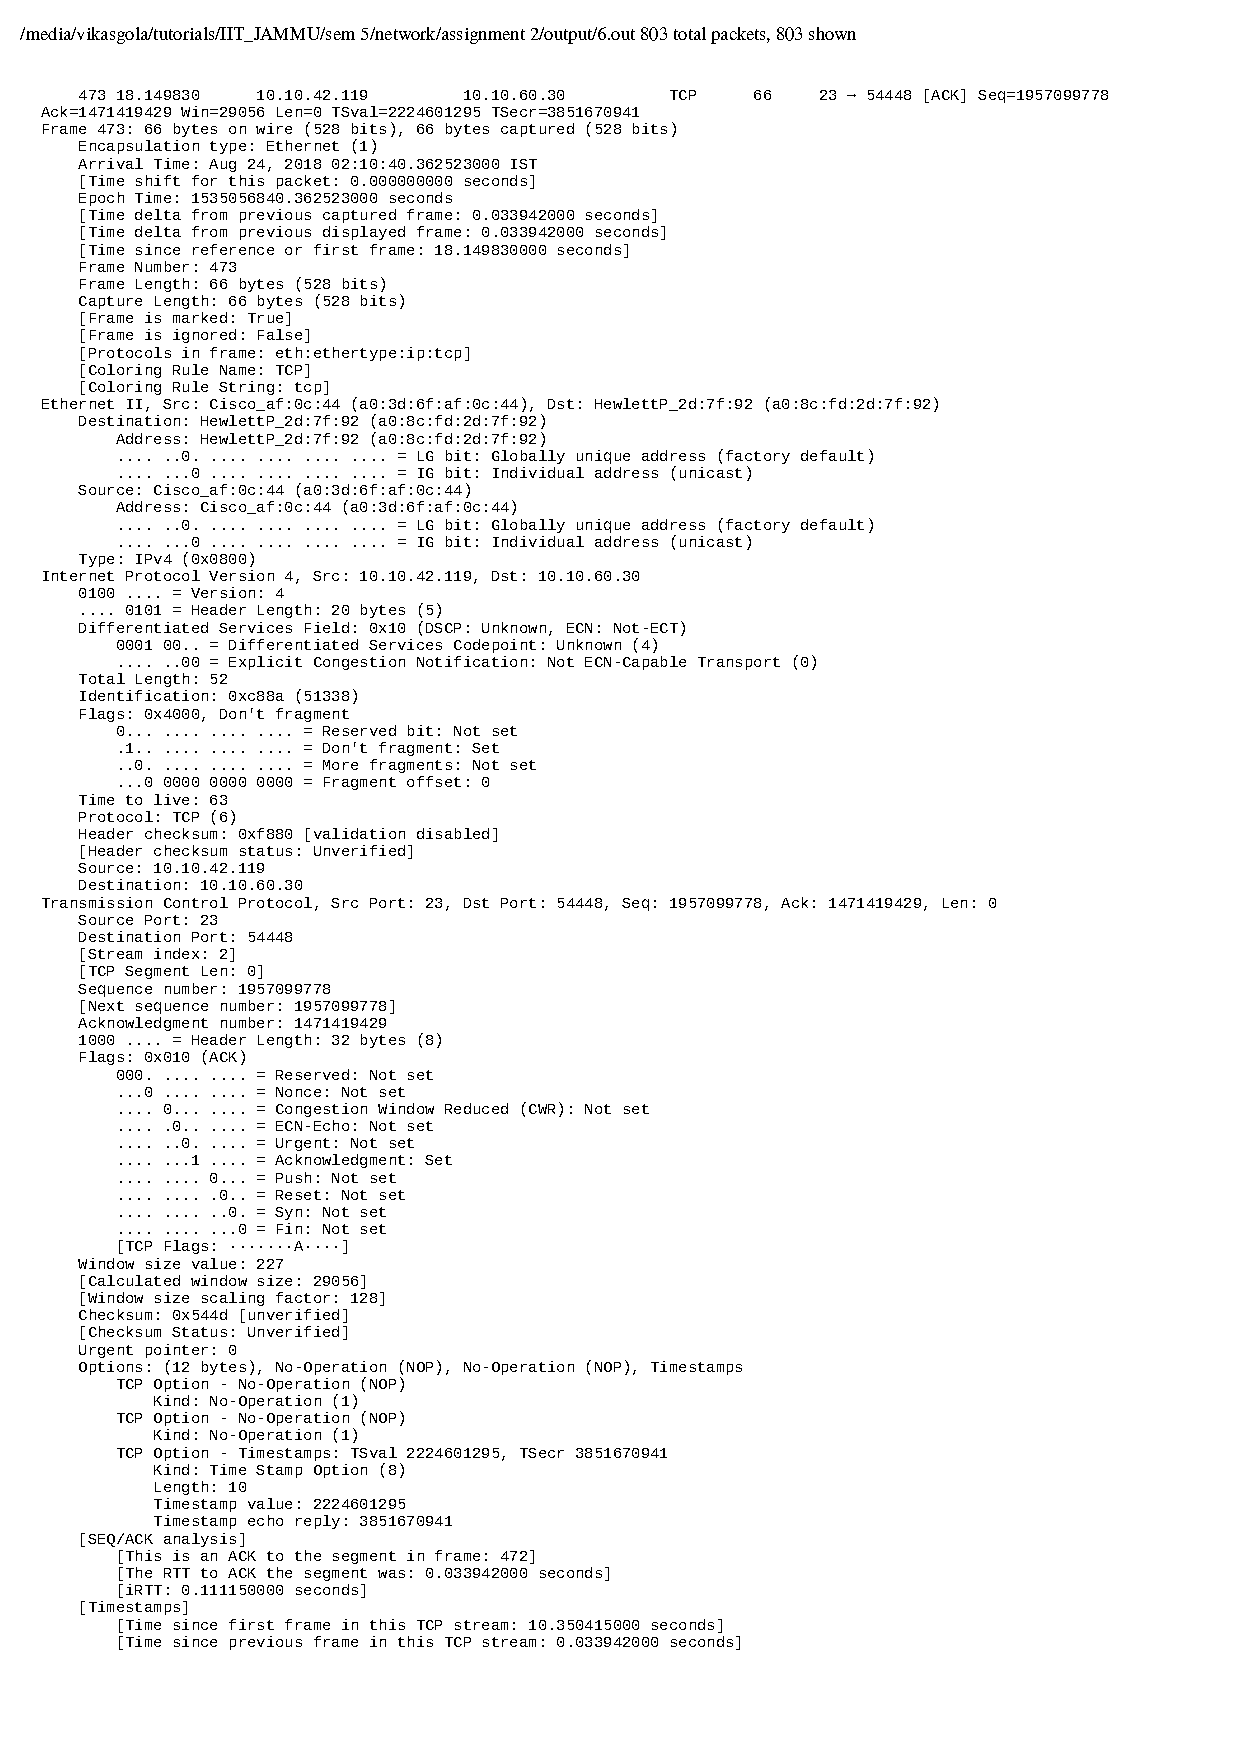
\includepdf[pages=-]{./output/6.pdf}
    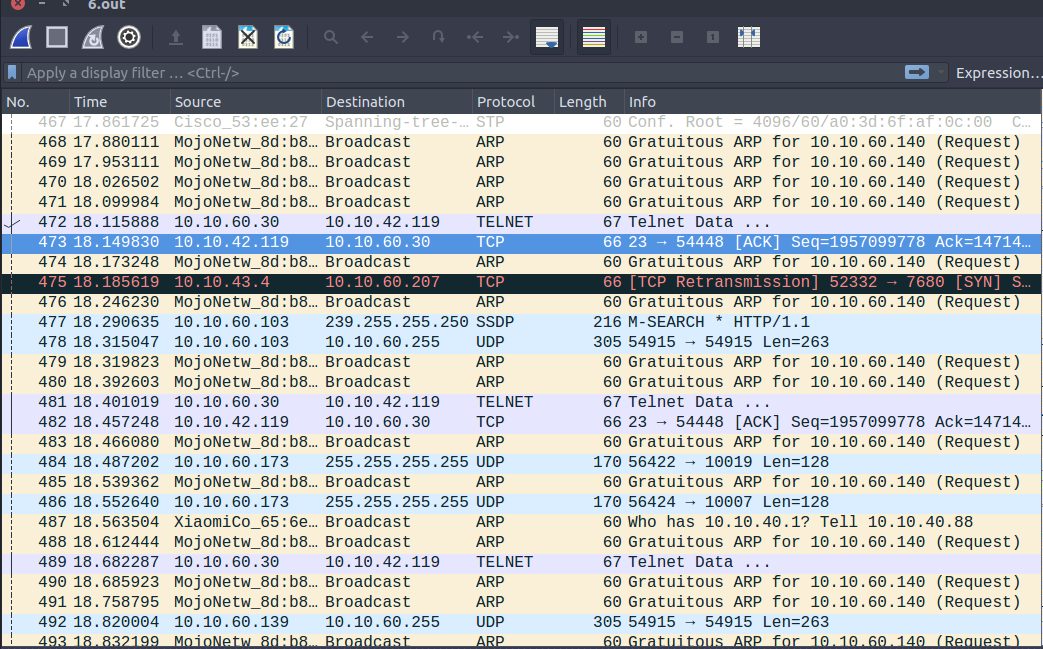
\includegraphics[scale=0.45]{6a}

    \vspace{1cm}


    \noindent
    \textbf{\large Question 7}
    In a manner similar to the previous exercise, now run tcpdump to capture an ARP request and an ARP
    reply and then use wireshark to analyze the frames. If there are no arp requests and replies in the
    network, generate some using arping a remote machine. After you see several ARP replies in the arping
    output, terminate the arping and the tcpdump program. Open the tcpdump trace using Wireshark -r
    exe7.out \&. Print one ARP request and one ARP reply using wireshark. Now answer the following
    questions:
    \begin{itemize}
        \item What is the value of the frame type field in an Ethernet frame carrying an ARP request and in an
        Ethernet frame carrying an ARP reply, respectively?
        \item What is the value of the frame type field in an Ethernet frame carrying an IP datagram captured
        in the previous exercise?
        \item What is the use of the frame type field?
    \end{itemize}
    \textbf{\large Answer}
    The printed ARP reply and request has been included in pdf you can check them in next pages 12(reply) and 13(request). 
    \begin{itemize}
        \item The value of the frame type field in Ethernet frame of an ARP request and reply are ARP(0x0806),ARP(0x0806) respectively.
        \item The value of the frame type field in an Ethernet frame carrying an IP datagram is IPv4(0x0800).
        \item The frame type field is use to payload of the internet frame and help recognizing the protocols.
    \end{itemize}
    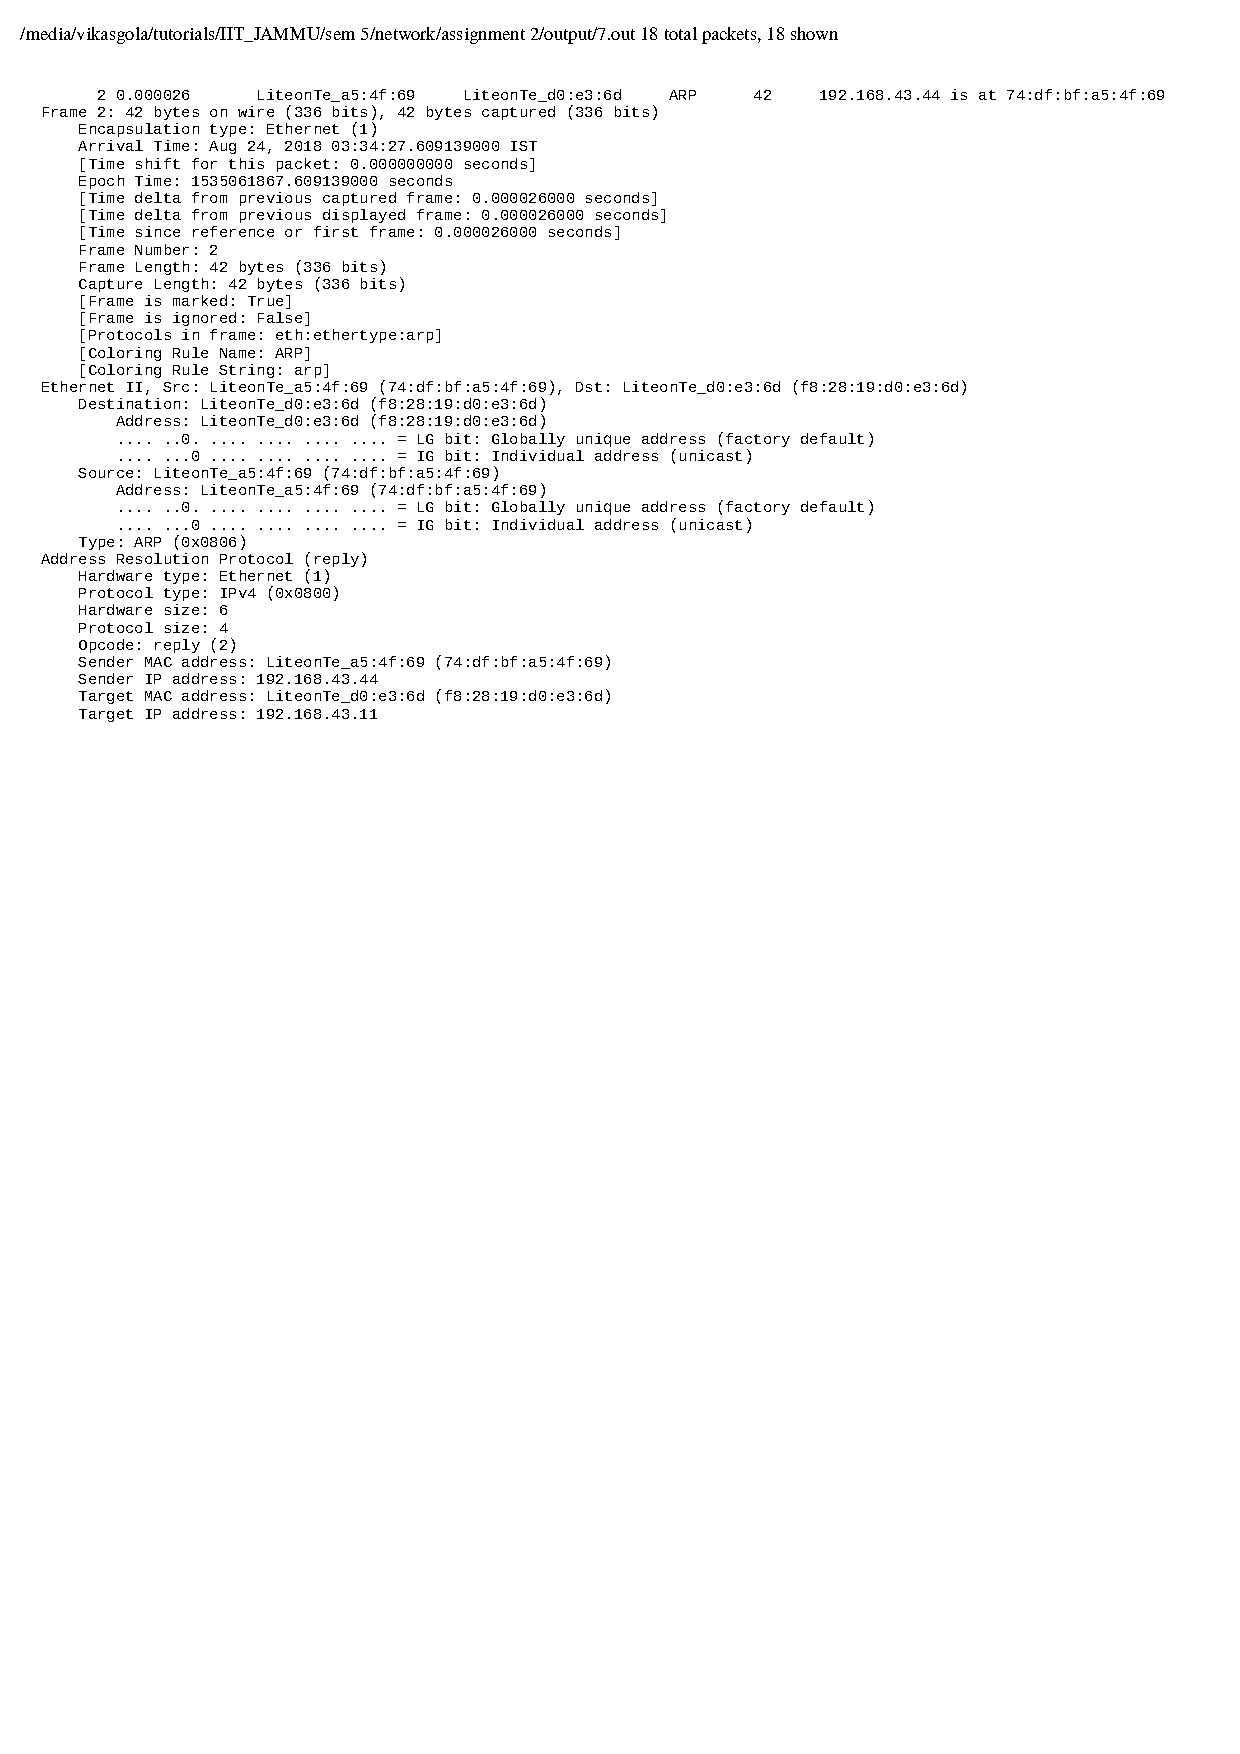
\includepdf[pages=-]{./output/7reply.pdf}
    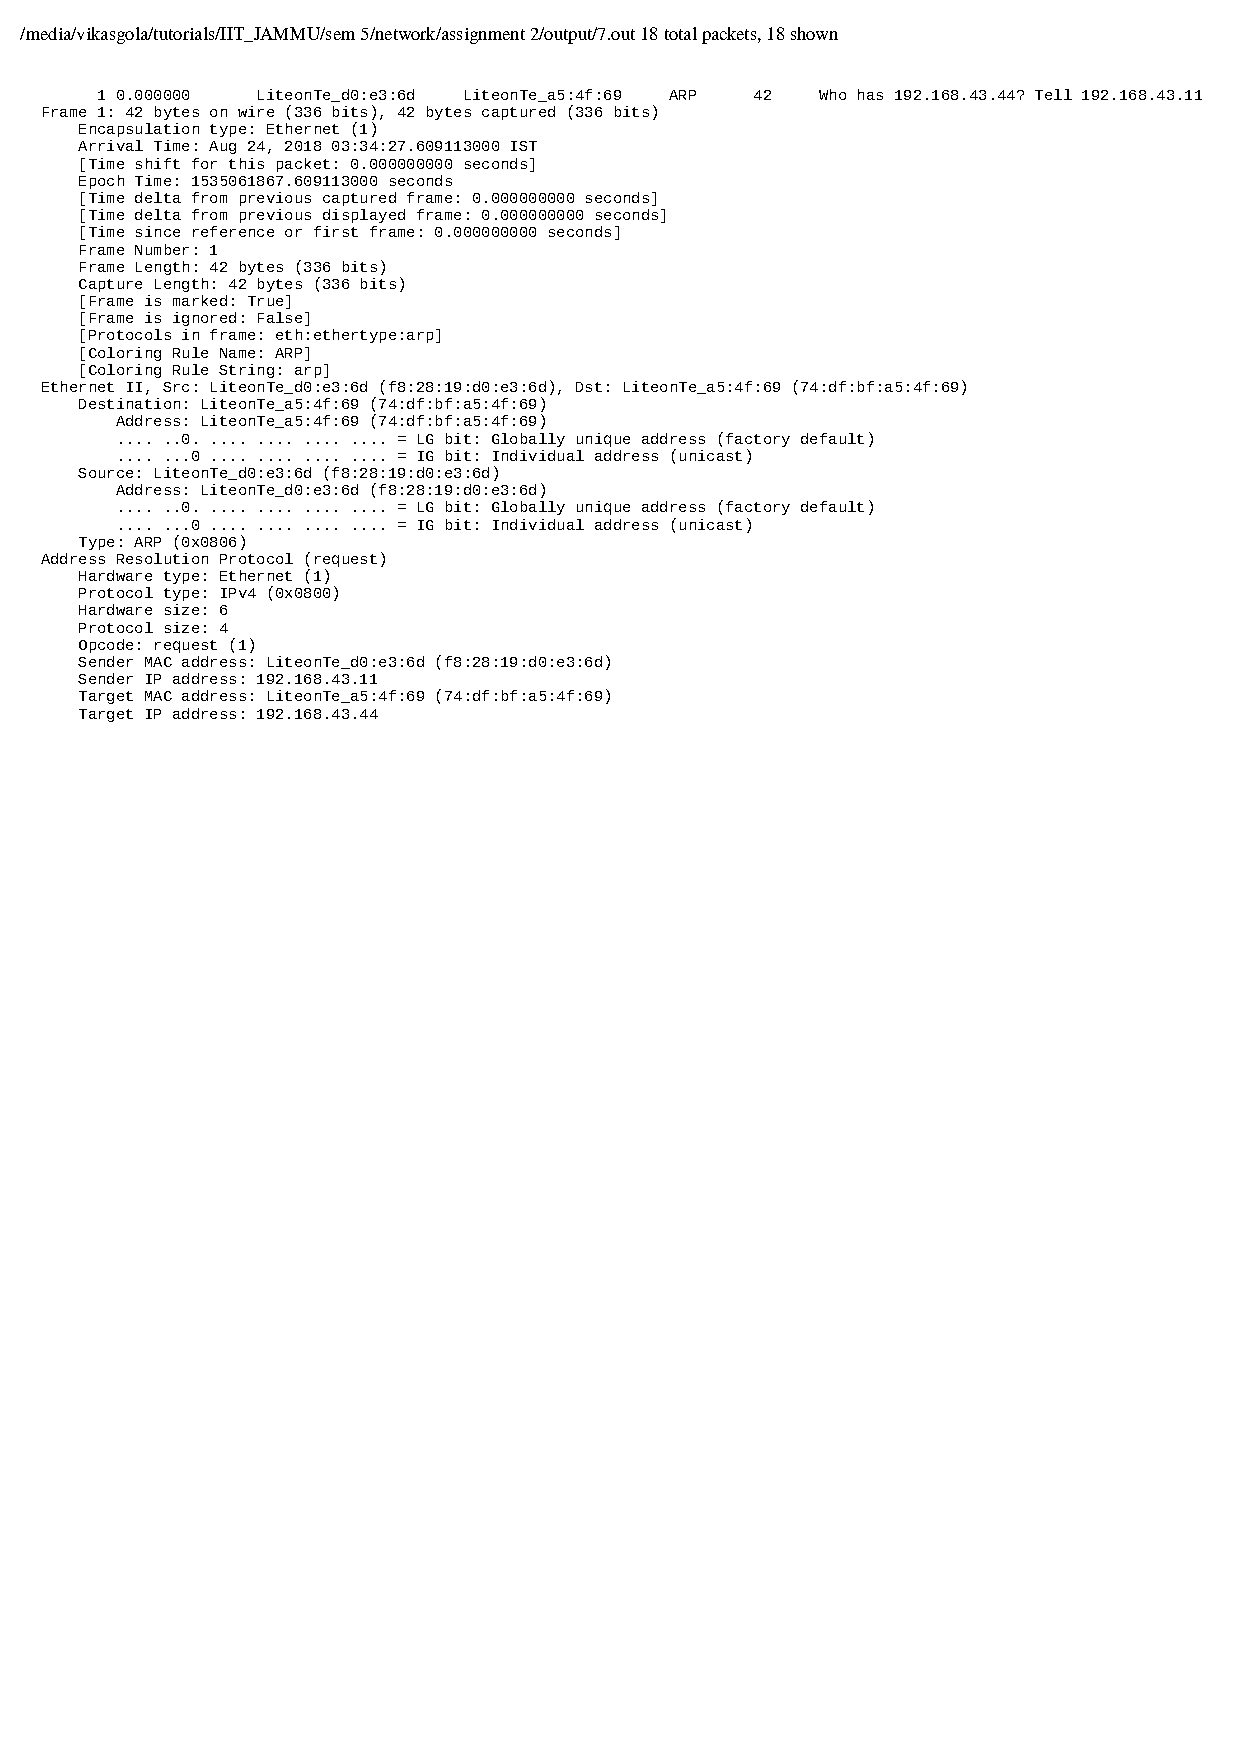
\includepdf[pages=-]{./output/7request.pdf}
    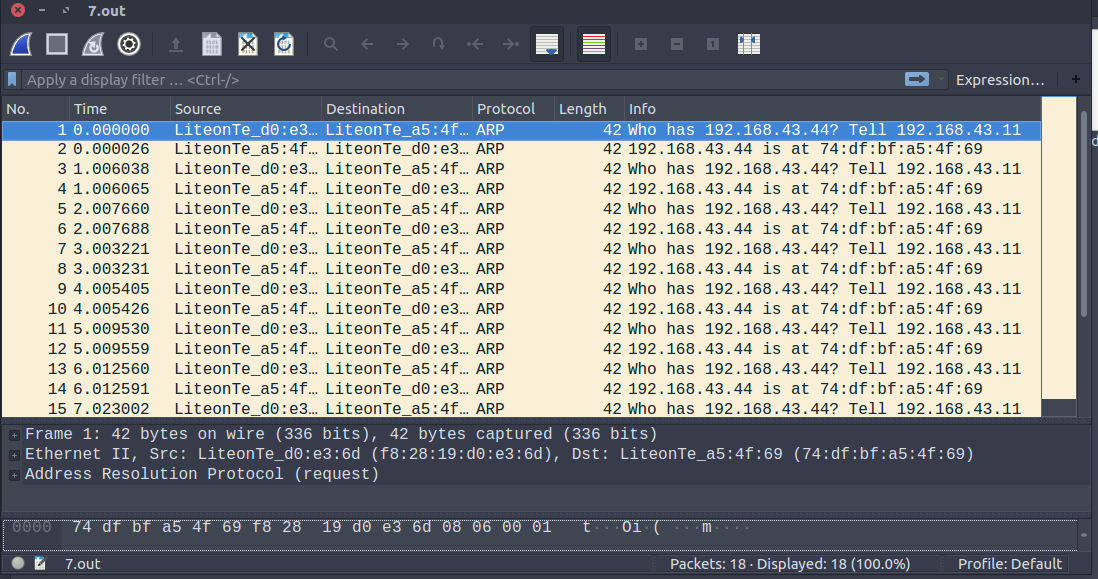
\includegraphics[scale=0.42]{7}
    \vspace{1cm}

    \noindent
    \textbf{\large Question 8}
    Explain briefly the purposes of the following tcpdump expressions.
    \begin{itemize}
        \item tcpdump udp port 520
        \item tcpdump -x -s 120 ip proto 89
        \item tcpdump -x -s 70 host ip addr1 and (ip addr2 or ip addr3)
        \item tcpdump -x -s 70 host ip addr1 and not ip addr2
    \end{itemize}
    \textbf{\large Answer}
    \begin{itemize}
        \item This command \textsf{tcpdump udp port 520} is use to capture UDP packets on port number 520.
        \item The command \textsf{tcpdump -x -s 120 ip proto 89} is use to truncated packet to 120 byte and print the data of packet with header
        \item This command \textsf{tcpdump -x -s 70 host ip addr1 and (ip addr2 or ip addr3)} is use capture packet which have host ip addr1 and remote host ip addr2 or remote host ip addr3 
        and also use to truncated packet to 70 with print data of the packet with header.
        \item This command \textsf{tcpdump -x -s 70 host ip addr1 and not ip addr2} is use capture packet which have host ip addr1 and remote host not ip addr2
        and also use to truncated packet to 70 with print data of the packet with header.
    \end{itemize}
    \vspace{1cm}

    \noindent
    \textbf{\large Question 9}
    Start tcpdump in a command window to capture packets between your machine and a remote host using:
    tcpdump -n -nn host your host and remote host. Execute a TCP utility, telnet for example - as in the
    problem before, in another command window. When you see a TCP packet in the tcpdump output,
    terminate tcpdump and save its output. Now answer the following question:
    \begin{itemize}
        \item What are the port numbers used by the remote and the local computer?
        \item Which machine port's port number matches the port number listed for telnet in the /etc/services file?
    \end{itemize}
    \textbf{\large Answer}
    \begin{itemize}
        \item The port numbers of remote and local computer are 23 and 46434 respectively.
        \item The port number of remote computer which is port 23 match with port number of telnet in /etc/services.
    \end{itemize}
    \vspace{1cm}

    \noindent
    \textbf{\large Question 10}
    Start tcpdump in one command window using tcpdump -n -nn host your host and remote host. Then,
    telnet to the remote host from a second command window by typing telnetremote h ost. Again issue
    the same telnetremote h ost command from a third command window. Now you are opening two telnet
    sessions to the same remote host simultaneously, from two different command windows. Check the port
    numbers being used on both sides of the two connections from the output in the tcpdump window. Save
    a TCP packet from each of the connections. Now answer the following questions:

    \begin{itemize}
        \item When you have two telnet sessions with your machine, what port number is used on the remote
        machine? Are both sessions connected to the same port number on the remote machine?
        \item What port numbers are used in your machine for the first and second telnet, respectively?
        \item What is the range of Internet-wide well-known port numbers? What is the range of well-known port
        numbers for Unix/Linux specific service? What is the range for a client port number? Compare
        your answer to the well-known port numbers defined in the /etc/services file. Are they consistent?
        In case they are not, try to discuss amongst peers and specify your view of the reason why they are
        not.
    \end{itemize}
    \textbf{\large Answer}
    \begin{itemize}
        \item Yes, both sessions of telnet connected to same port number on remote host that is 23.
        \item 46686 and 46688 port numbers are used in my machine in first and second telnet sessions.
        \item The range of well known port numbers is 0 to 1023.
        The range of unix/linux specific services is 512 to 995.
        The range of client port number is 49152 to 65535.
        Yes, they are consistent.
    \end{itemize}
    
    \vspace{1cm}

\end{document}